\section{Game Characterization of Cycle Rank}

\subsection{Definitions}
\paragraph{}
For this section, we will assume all our graphs are directed and contain no self loops. We will also need some basic definitions before we can start talking about the games we will use to define cycle rank.
\begin{description}
 \item[Successor-closed] \hfill \\
H $\subseteq$ $G$ is an successor-closed of $G$ if $H$ is there are no edges from $H$ to $G \setminus H$.
\item[String] \hfill \\
A string is a sequencce of elements $a_1, \ldots, a_n$ such that all $a_i$ belong to the same set. That set is called the alphabet.
\item[Length] \hfill \\
The lenght of a string  A = $a_1, \ldots, a_n$, denoted by $|$A$|$ is n. The length of the empty string is 0.
\item[Concatenation] \hfill \\
The concatenation of two string A =  $a_1, \ldots, a_n$ and B =  $b_1, \ldots, b_k$, denoted by A$\cdot$B is $a_1, \ldots, a_n,b_1, \ldots, b_k$
\item[V*] \hfill \\
V* is the set of all possible finite words over the set V, including the empty word.
\item[Prefix] \hfill \\
X $\in$ V* is a prefix of Y $\in$ V*, denoted by X$\preceq$Y  if Z $\in$ V* exists such that Y = X$\cdot$Z.
\item[String to set] \hfill \\
For a string S = $a_1, \ldots, a_n$, $\{|S|\}$ denotes the set $\{a_1, \ldots, a_n\}$.
\item[Symmetric difference] \hfill \\
For two sets A and B their symmetric difference, expressed as A$\Delta$B is (A$\cup$B)\textbackslash (A $\cap$B).
\end{description}

\subsection{Game description}
\paragraph{Informal definition:}
We will use a cops and robbers game played on a graph G, where the cops will try to catch a robber. In each step of the game the cops can either place a cop on a node or remove only the most recently placed one. This is why it's called a LIFO search. The cops win if the manage to place a cop in the same node where the robber is.

The are four variants of the game depending on how the robber moves and which information do the cops have. 
\begin{description}
\item[Invisible - i] \hfill \\
The cops don't know the position where the robber is located and he can move along directed paths in G that contain no cops.
\item[Visible - v] \hfill \\
The cops know the position where the robber is located and he can move along directed paths in G that contain no cops.
\item[Invisible strongly connected - isc] \hfill \\
The cops don't know the position where the robber is located and he can only move inside the same strongly connected component of G that contain no cops.
\item[Visible strongly connected - isc] \hfill \\
The cops know the position where the robber is located and he can only move inside the same strongly connected component of G that contain no cops.
\end{description}

\paragraph{Formal definition:}
For a digraph G, the state of the game is described by a pair (X, R). X $\in$ V* is the position of the cops and the order in which they were added. R is an induced subgraph of G\textbackslash \{$|$X$|$\}. In the invisible variants, R represents where the robber may be, while in the visible variants its means which nodes can the robber reach. We will define the valid states for each game variant.

\begin{description}
\item[i-state] \hfill \\
R is successor closed in G\textbackslash \{$|X|$\}. If R wouldn't be successor closed the robber would have an edge without cops which he could use to scape R and R wouldn't represent all possible positions of the robber.
\item[v-state] \hfill \\
R is successor closed in G\textbackslash \{$|X|$\} and $v \in$ V($R$) exists such that a directed path exist from $v$ to any other node in V($R$).
\item[isc-state] \hfill \\
R is a union of strongly connected components of $G \setminus$ \{$|X|$\}.
\item[vsc-state] \hfill \\
R is a single strongly connected component of $G \setminus$ \{$|X|$\}.
\end{description}

Let ($X$, $R$) be the current state of the game and ($X'$, $R'$) a valid successor (a possible next state). Then, $| \{|X|\} \Delta \{|X'|\}| = 1$ and $|X|\preceq |X'|$ or $|X'|\preceq |X|$. R is defined differently for different game variants.
\begin{itemize}
\item In the i and v variants, for every $v' \in V(R')$ there exists a $v \in V(R)$ such that a path exists from $v$ to $v'$ in $G$ $\setminus (\{|X|\} \cap \{|X'|\}|).$
\item In the isc and vsc variants, for every $v' \in V(R')$ there exists a $v \in V(R)$ such that $v$ and $v'$ are contained in the same strongly connected component of $G \setminus (\{|X|\} \cap \{|X'|\}|).$
\end{itemize}

The initial state of a game in the invisible variants is clearly ($\epsilon$, $G$). In the visible variants this is not necessarily a valid state, so the initial state will be any valid position of the form ($\epsilon$, $R$). A strategy for the cops is a function that given a game state (X, R) returns X', the position the cops will take in the next state. A strategy is said to be a winning strategy if no matter which moves the robber makes the strategy reaches a state of the form (X, $\emptyset$) from any possible initial state.

\paragraph{}
For every previously mentioned game variants we can create a new monotone variant (mi, mv, misc, mvsc). The monotone variant of each game is equal to the non monotone one, except that for every position ($X_i$, $R_i$) and its successor ($X_{i+1}$, $R_{i+1}$), the cops strategy must assure that $R_{i+1}$ is a subgraph of $R_i$ no matter what the robber does. 

\paragraph{}
We are interested in the minimum number of cops necessary to capture the robber. For any game variant, gv $\in$ \{i, v, isc, vsc, mi, mv, misc, mvsc\}, we will call LIFO$^{gv}$(G) the minimum number of cops needed to capture a robber in G in that game variant. We will also define one more game called searcher stationary vsc, which is equal to the LIFO vsc but for every $X_i$,$X_i \prec X_{i+1}$, i.e, cops can only be added, not removed. SS$^{vsc}$ will be the minimum number of cops needed in this strategy.

\begin{theorem}
For any digraph G the same number of cops are needed to capture a robber in every game variant and that number is equal to the cycle rank of G plus 1:

1 + r(G) = LIFO$^{mi}$(G) = LIFO$^{i}$(G) = LIFO$^{misc}$(G) = LIFO$^{isc}$(G) = LIFO$^{mv}$(G) = LIFO$^{v}$(G) = LIFO$^{mvsc}$(G) = LIFO$^{vsc}$(G) = SS$^{vsc}$(G).
\end{theorem}
\begin{observation} There are some trivial relations between these games\\
\begin{itemize}
\item Every monotone winning strategy is also a winning strategy in the non monote variant of that same game.
\item Every winning strategy for an invisible game variant is also a winning strategy for the visible variant of that same game.
\item Every winning strategy for when the robber is not restricted to only move in strongly connected components is also winning when the robber is restricted to only move in strongly connected components.
\end{itemize}
\end{observation}

With this observation we can build the following figure.

\begin{figure}[H]
\usetikzlibrary{arrows}
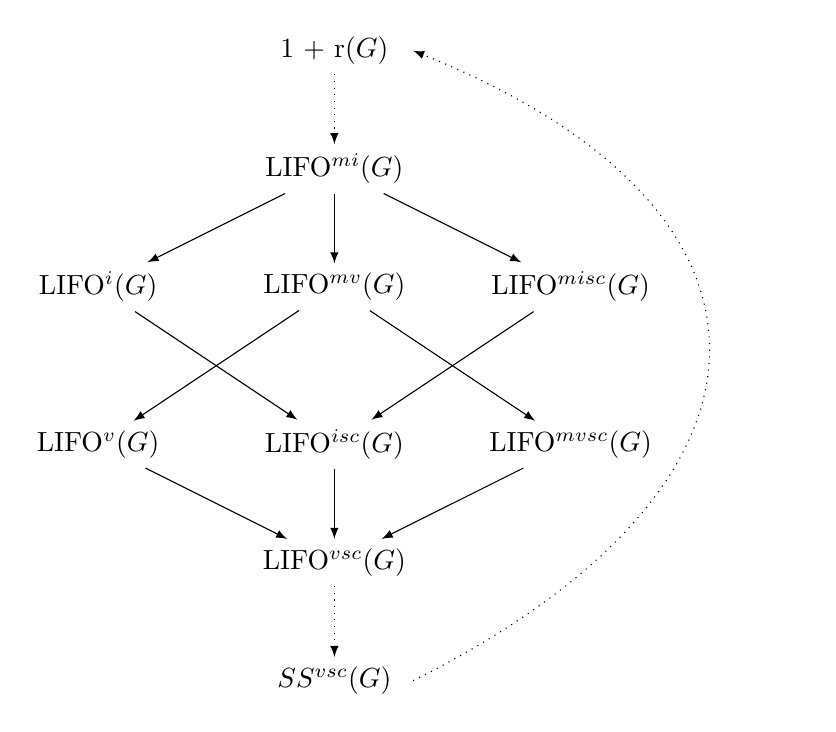
\begin{tikzpicture}

\node (v1) at (0,0) {LIFO$^{mi}(G)$};
\node (v2) at (-3,-1.5) {LIFO$^{i}(G)$};
\node (v3) at (0,-1.5) {LIFO$^{mv}(G)$};
\node (v4) at (3,-1.5) {LIFO$^{misc}(G)$};
\draw [-latex] (v1) edge (v2);
\draw [-latex] (v1) edge (v3);
\draw [-latex] (v1) edge (v4);
\node (v6) at (-3,-3.5) {LIFO$^{v}(G)$};
\node (v5) at (0,-3.5) {LIFO$^{isc}(G)$};
\node (v7) at (3,-3.5) {LIFO$^{mvsc}(G)$};
\draw [-latex] (v2) edge (v5);
\draw [-latex] (v4) edge (v5);
\draw [-latex] (v3) edge (v6);
\draw [-latex] (v3) edge (v7);
\node (v8) at (0,-5) {LIFO$^{vsc}(G)$};
\draw [-latex] (v6) edge (v8);
\draw [-latex] (v7) edge (v8);
\draw [-latex] (v5) edge (v8);
\node (v9) at (0,1.5) {1 + r($G$)};
\draw [dotted, -latex] (v9) edge (v1);
\node (v10) at (0,-6.5) {$SS^{vsc}(G)$};
\draw [dotted, -latex] (v8) edge (v10);

\draw [dotted, -latex](1,-6.5) .. controls (6,-4) and (6,-0.5) .. (1,1.5);
\end{tikzpicture}
\caption{The arrows go from the bigger values to the smaller ones. We have the normal arrows from the previous observation. We will prove the doted arrows and that will prove that the lemma holds.}
\end{figure}


\begin{lemma}
For any digraph G, LIFO$^{vsc}$(G) $\geq$ SS$^{vsc}$(G).
\end{lemma}
@@TODO
\begin{proof}
We will proof this by contradiction. Lets assume state ($X$, $R$) and a winning strategy $f$ for the LIFO game variant exist such that, $f$($X$, $R$) = $X'$, $|X'| < |X|$ and $|R|$ > 1. We will proof that the cops can't win with such an strategy. Define $R' \subset R$ such that ($X'$, $R'$) is a valid successor of ($X$, $R$).
\end{proof}
\begin{lemma}
For any digraph G, SS$^{vsc}$(G) $\geq$ 1 + r($G$).
\end{lemma}
\begin{proof}
We will prove this by induction over the number of vertices of $G$.
\begin{enumerate}
  \item If $|$V($G$)$|$ = 1, SS$^{vsc}$(G) = 1 + r($G$) = 1. \\
  PROOF: A cop in the single node of G will always capture the robber and $|$V($G$)$|$ = 1, so r($G$) = 0 by definition.
  \item Assume that for every G' such that  $|$V(G')$| < |$V(G)$|$, SS$^{vsc}$($G'$) $\geq$ 1 + r($G'$). \\
  PROOF: Induction hypothesis, we can assume it because 1.
  \item If G is not strongly connected, then SS$^{vsc}$($G$) $\geq$ 1 + r($G$)
  \begin{enumerate}[label*=\arabic*.]
    \item G has k $>$ 1 strongly connected components $H_1, \ldots, H_k$ and for every $H_i$, $|$V($H_I$)$| < |$V(G)$|$. \\
    PROOF: In 3 we assume G is not strongly connected.
    
    \item SS$^{vsc}$(G) $\geq$ SS$^{vsc}$($H_i$) such that $H_i$ is a strongly connected component of G. \\
    PROOF: SS$^{vsc}$(G) must have a winning strategy for any strongly connected component the robber may start in.
    
    \item $\max_{H_i}$ SS$^{vsc}$($H_i$) $\geq$  $\max_{H_i}$ (1 + r($H_i$)). \\
    PROOF: By 2 and 3.1.
    
    \item SS$^{vsc}$(G) $\geq$ $\max_{H_i}$ SS$^{vsc}$($H_i$) $\geq$  $\max_{H_i}$ (1 + r($H_i$)) = 1 + r(G). \\
    PROOF: The first equality by 3.2. The second inequality by 3.3. The last one by definition of cycle rank.
  \end{enumerate}
  \item If G is strongly connected, then SS$^{vsc}$(G) $\geq$ 1 + r(G) 
  \begin{enumerate}[label*=\arabic*.]
    \item Let $\phi$ be a minimal strategy, that uses SS$^{vsc}$(G) cops and v = \{$|\phi$($\epsilon$, G)$|$\}. \\
    PROOF: By 4, ($\epsilon$, G) is the initial state, so v exists.
    
    \item SS$^{vsc}$(G) = 1 + SS$^{vsc}$(G - v). \\
    PROOF: By 4.1 $\phi$ induces a winning strategy for SS$^{vsc}$(G - v) using SS$^{vsc}$(G)-1 cops.
    
    \item SS$^{vsc}$(G) = 1 + SS$^{vsc}$(G - v) $\geq$ 2 + r(G-v) $\geq$ 1 + r(G). \\
    PROOF: The first inequality by 4.2. The second inequality by 2. The last one is by the definition of cycle rank, as r(G) is the smallest r(G-u) + 1, then 1+ r(G-u) $\geq$ r(G) for any u $\in$ V(G).
  \end{enumerate}
  \item Q.E.D. \\
  PROOF: By 3 and 4.
\end{enumerate}
\end{proof}

\begin{lemma}
1 + r(G) $\geq$ LIFO$^{mi}$(G)
\end{lemma}
\begin{proof}
We will prove this by induction over the number of vertices of G.
\begin{enumerate}
  \item If $|$V(G)$|$ = 1, LIFO$^{mi}$(G) = 1 + r(G) = 1. \\
  PROOF: A cop in the single node of G will always capture the robber and $|$V(G)$|$ = 1, so r(G) = 0 by definition.
  \item Assume that for every G' such that  $|$V(G')$| < |$V(G)$|$, 1 + r(G') $\geq$ LIFO$^{mi}$(G'). \\
  PROOF: Induction hypothesis.
  \item If G is strongly connected, 1 + r(G) $\geq$ LIFO$^{mi}$(G).
  \begin{enumerate}[label*=\arabic*.]
    \item v $\in$ V(G) exists, such that r(G) = 1+ r(G-v). \\
    PROOF: By definition of cycle rank.
    \item 1 + LIFO$^{mi}$(G-v) $\geq$ LIFO$^{mi}$(G). \\
    PROOF: We can place a cop in v in the first step of the game, never remove it and win the game in G using 1 + LIFO$^{mi}$(G-v) cops.
    \item  1 + r(G) = 2 + r(G-v) $\geq$ 1 + LIFO$^{mi}$(G-v) $\geq$ LIFO$^{mi}$(G). \\
    PROOF: By 3.1, 2 and 3.2
  \end{enumerate}
  \item If G is not strongly connected, 1 + r(G) $\geq$ LIFO$^{mi}$(G).
  \begin{enumerate}[label*=\arabic*.]
    \item G has k $>$ 1 strongly connected components $H_1, \ldots, H_k$ and for every $H_i$, $|$V($H_i$)$| < |$V(G)$|$. \\
    PROOF: In 4 we assume G is not strongly connected.
    \item A strongly connected component $H_i$ exists such that there is no edge from $G\setminus H_i$ to $H_i$. \\
    PROOF: By 4.1 G is not strongly connected, so $H_i$ must exist.
    \item LIFO$^{mi}$(G) $\geq$ max(LIFO$^{mi}$($G\setminus H_i$), LIFO$^{mi}$($H_i$)). \\
    PROOF: The cops can search the robber only in $H_i$. Then, they can remove every cop in $H_i$ and search only in $G\setminus H_i$. The robber will never be able to go back to $H_i$ because of 4.2
    \item LIFO$^{mi}$(G) $\geq$ max(LIFO$^{mi}$($G\setminus H_i$), LIFO$^{mi}$($H_i$)) $\geq$ max(1+r($G\setminus H_i$), 1 + r($H_i$)) = 1 + r(G). \\
    PROOF: The first inequality by 4.3. The second one by 2. The last equality by the definition of cycle rank and the assumption that G is not strongly connected.
  \end{enumerate}ç
  \item Q.E.D. \\
  PROOF: By 3 and 4.
\end{enumerate}
\end{proof}